\documentclass[xcolor=svgnames,aspectratio=169]{beamer}
\usetheme{Boadilla}

\usepackage[utf8]{inputenc}
\usepackage[T1]{fontenc}
\usepackage{lmodern}
\usepackage[whole]{bxcjkjatype}
\usepackage[backend=biber]{biblatex}
\addbibresource{octave.bib}
\usepackage{mathtools}
\usepackage{multimedia}
\usepackage{siunitx}
\usepackage{pifont}
\usepackage{tikz}
\newcommand*\colorcheck[1]{%
  \expandafter\newcommand\csname #1check\endcsname{\textcolor{#1}{\ding{52}}}%
}
\colorcheck{green}

\title[GNU Octave]{Scientific programming with GNU Octave
  
\includegraphics[width=1.5em]{res/images/octave-logo-1024.png}
}
\author[Kai T. Ohlhus]{
  オールフス カイトーベン \\
  OHLHUS, Kai Torben}
\institute[TWCU]{
  理学研究科 \\
  Graduate School of Science \\
  東京女子大学 \\
  Tokyo Woman's Christian University}
\date{December 24, 2019}
\titlegraphic{
\vfill
\hfill
\includegraphics[height=1em]{res/images/cc-by-sa}
}

\begin{document}

{
\usebackgroundtemplate{
  \vbox to \paperheight{\vfil\hbox to \paperwidth{\hfil
  \tikz\node[opacity=0.15] {
  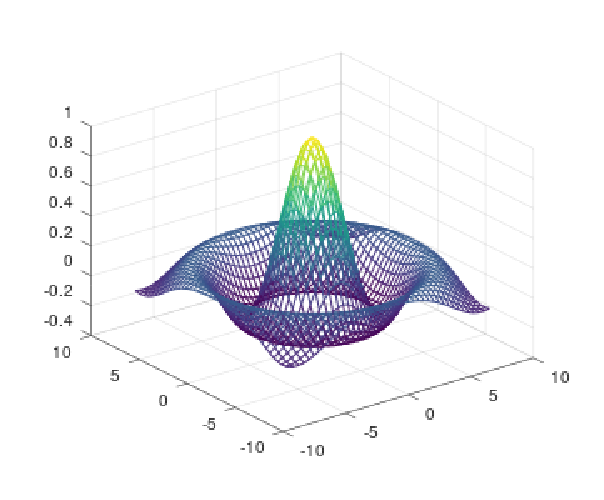
\includegraphics[width=0.6\paperwidth]{res/images/example-mesh}
  };
  \hfil}\vfil}
}
\frame{\titlepage}
}


\section{Installation}
\frame{\tableofcontents[currentsection]}
\begin{frame}{Installing GNU Octave on MS Windows 10 (1/8)}
\begin{center}
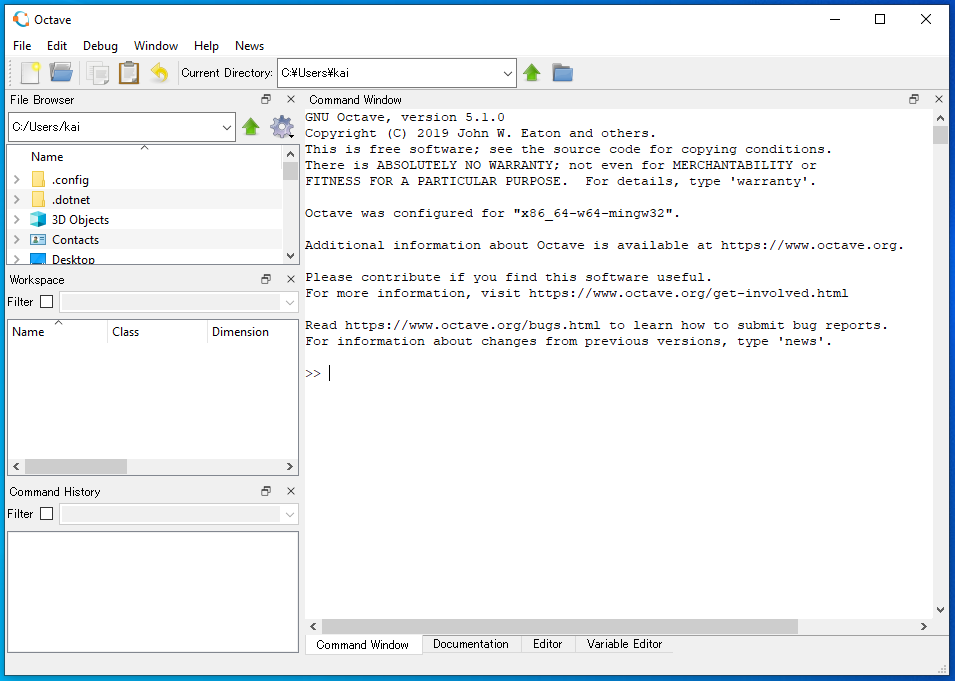
\includegraphics[width=0.65\textwidth]{res/ms_windows/win_octave_gui.png}
\end{center}
\end{frame}



\begin{frame}{Installing GNU Octave on MS Windows 10 (2/8)}
\begin{columns}
\begin{column}{0.35\textwidth}
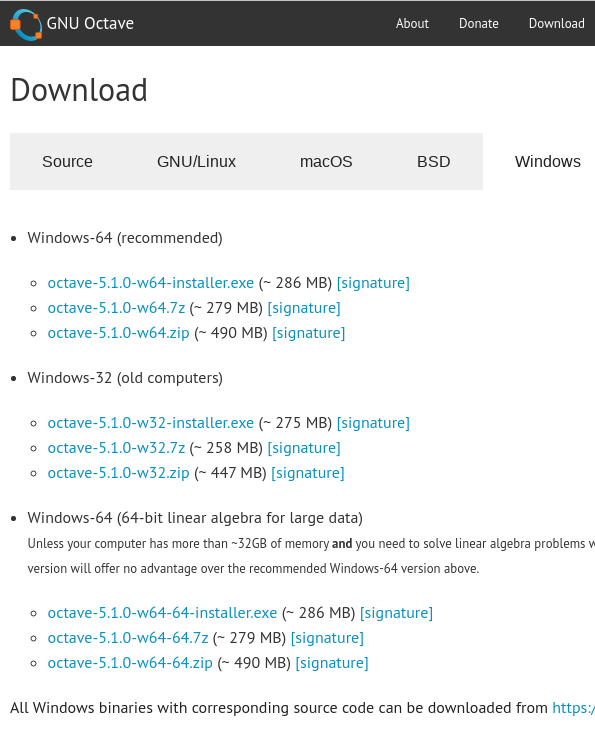
\includegraphics[width=\textwidth]{res/ms_windows/win_download_cropped.png}
\end{column}
\begin{column}{0.6\textwidth}
{\Large\color{DarkBlue}\url{https://www.octave.org/download}}\\[1em]

\begin{itemize}
\itemsep1em
\item
\textbf{w32}: 32-bit systems (very old or embedded devices)

\item
\textbf{w64}: 64-bit systems \greencheck

\item
\textbf{w64-64}: 64-bit systems with \textbf{large} main memory:\\[1em]
\begin{itemize}
\item
Objects with more than $2^{32}$ Elements, e.g.\\[1em]

$\num{66000}\times\num{66000}$-matrices (dense)\\[1em]

$\approx\mathbf{32 \,GB}$ (double precision)
\end{itemize}
\end{itemize}
\end{column}
\end{columns}
\end{frame}



\begin{frame}{Installing GNU Octave on MS Windows 10 (3/8)}
\begin{columns}
\begin{column}{0.35\textwidth}
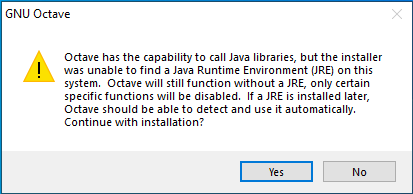
\includegraphics[width=\textwidth]{res/ms_windows/win_install_java_warning.png}
\end{column}
\begin{column}{0.5\textwidth}
\textbf{Ignore} Java warning:
\begin{itemize}
\item
Octave works perfectly without Java.

\item
Octave's Java interface might not work properly.
\end{itemize}
\end{column}
\end{columns}
\bigskip
\begin{columns}
\begin{column}{0.35\textwidth}
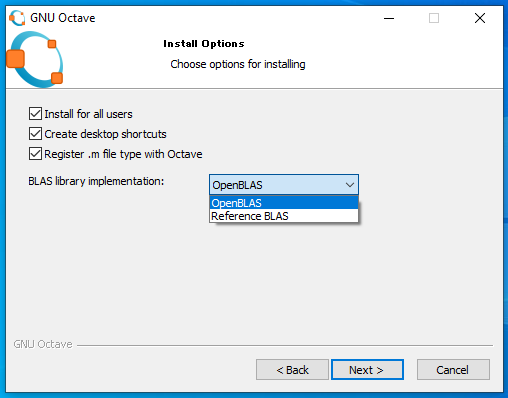
\includegraphics[width=\textwidth]{res/ms_windows/win_install_blas.png}
\end{column}
\begin{column}{0.5\textwidth}
\textbf{Choose:}
\begin{itemize}
\item
{\color{DarkBlue}OpenBLAS} (usually faster)

{\footnotesize \url{https://www.openblas.net/}}

\item
{\color{DarkBlue}Reference BLAS}

{\footnotesize \url{https://www.netlib.org/blas/}}
\end{itemize}
\end{column}
\end{columns}
\end{frame}



\begin{frame}{Installing GNU Octave on MS Windows 10 (4/8)}
\begin{columns}
\begin{column}{0.2\textwidth}
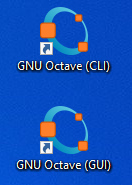
\includegraphics[width=\textwidth]{res/ms_windows/win_install_desktop_icons.png}
\end{column}
\begin{column}{0.3\textwidth}
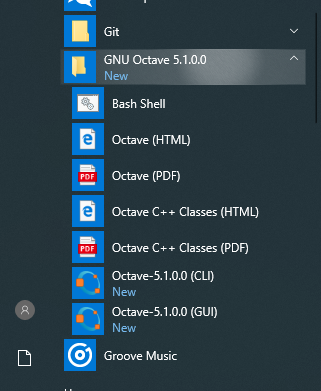
\includegraphics[width=\textwidth]{res/ms_windows/win_install_startmenu_icons.png}
\end{column}
\begin{column}{0.45\textwidth}
\begin{itemize}
\itemsep1em
\item
As usual, the installer creates
\begin{itemize}
\itemsep0.6em
\item
desktop icons (left)
\item
start menu entries (right)
\end{itemize}
\item
to start
\begin{itemize}
\itemsep0.6em
\item
\textbf{command-line interface (CLI)}
\item
\textbf{graphical user interface (GUI)}
\end{itemize}
\end{itemize}
\end{column}
\end{columns}
\end{frame}



\begin{frame}{Installing GNU Octave on MS Windows 10 (5/8)}
\begin{center}
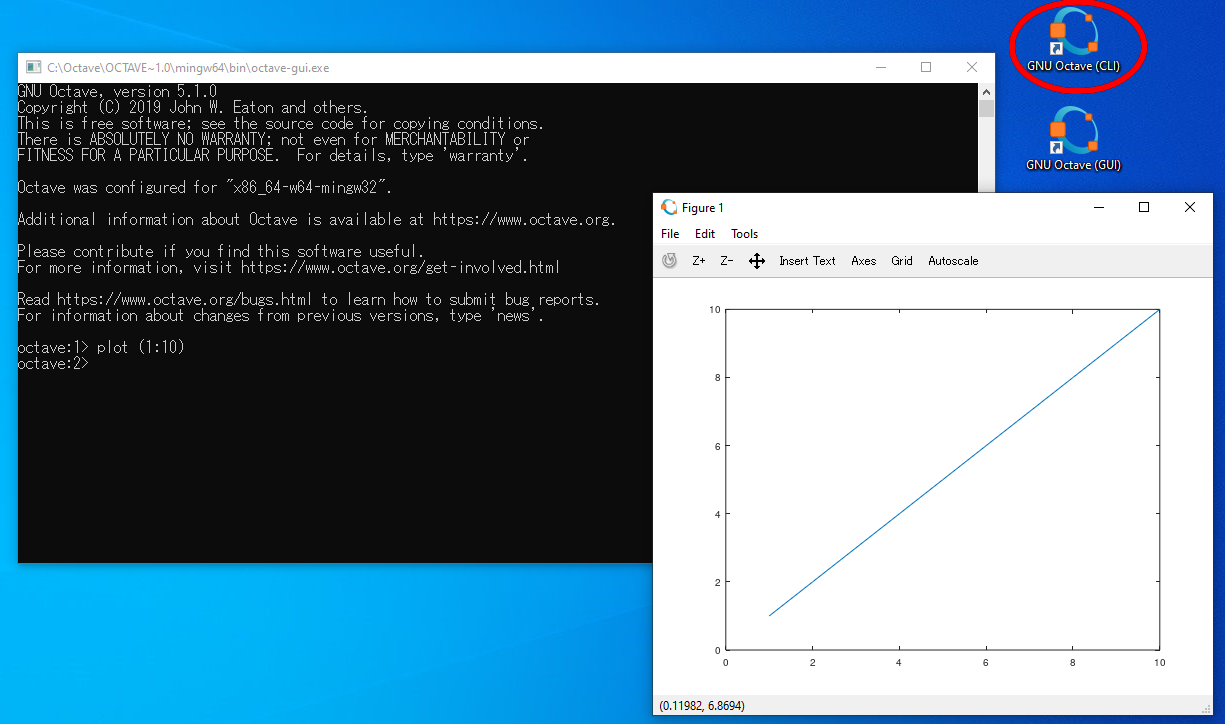
\includegraphics[width=0.75\textwidth]{res/ms_windows/win_octave_cli_plot.png}
\end{center}
\end{frame}



\begin{frame}{Installing GNU Octave on MS Windows 10 (6/8)}
\begin{center}
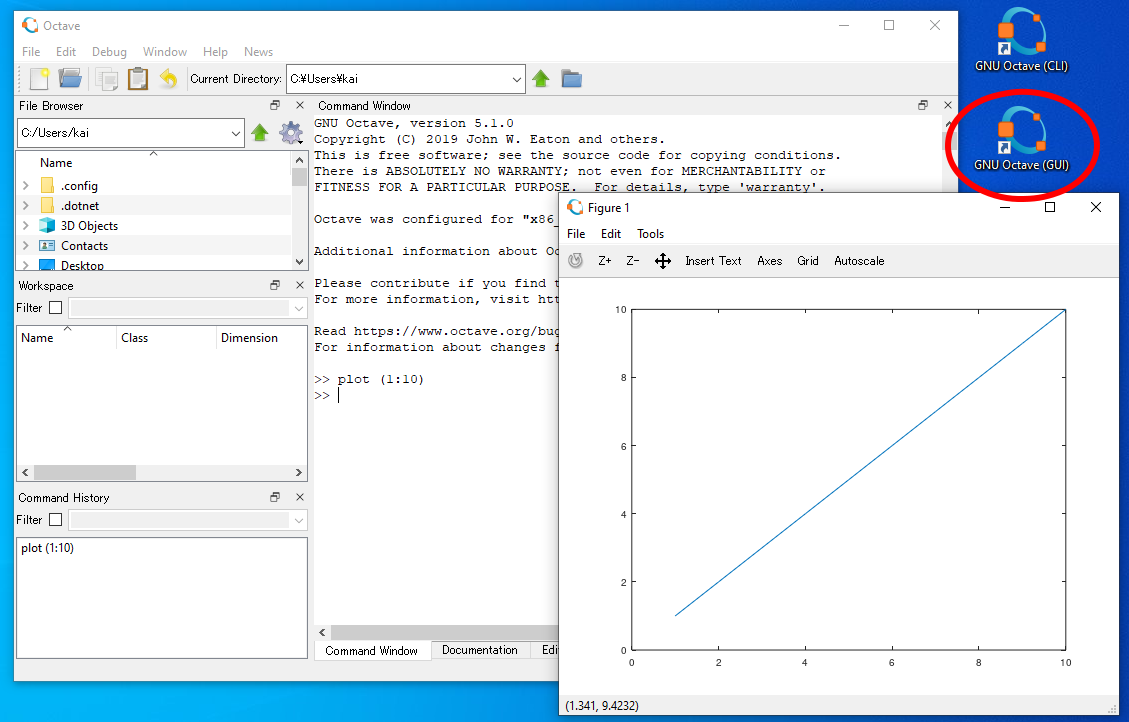
\includegraphics[width=0.7\textwidth]{res/ms_windows/win_octave_gui_plot.png}
\end{center}
\end{frame}



\begin{frame}{Installing GNU Octave on MS Windows 10 (7/8)}
\begin{columns}
\begin{column}{0.55\textwidth}
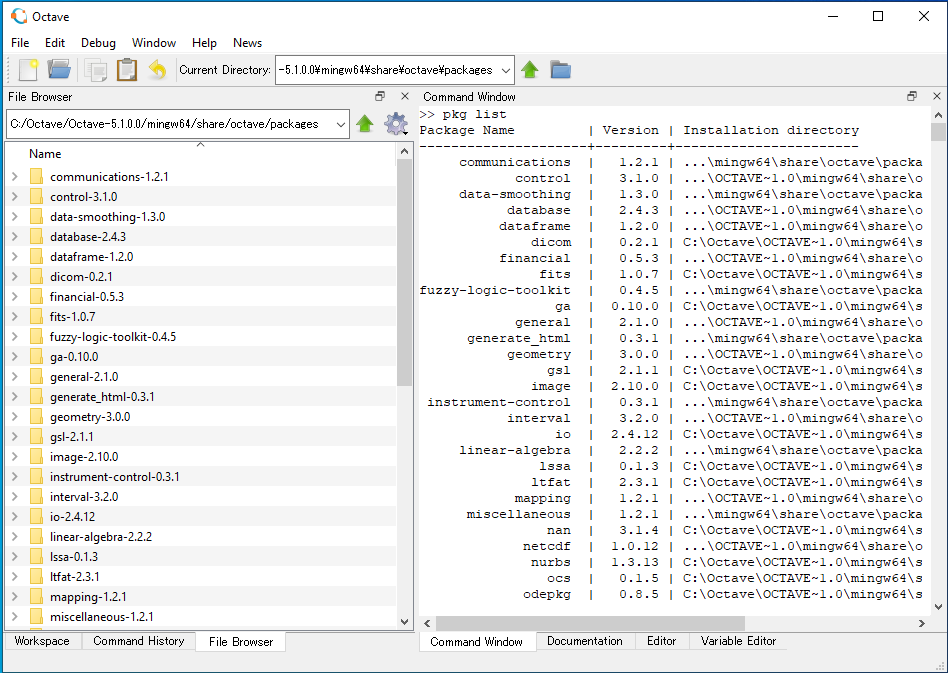
\includegraphics[width=\textwidth]{res/ms_windows/win_octave_packages.png}
\end{column}
\begin{column}{0.35\textwidth}
\begin{itemize}
\itemsep1em
\item
Many \textbf{\color{DarkBlue}Octave Forge} packages
already shipped precompiled as part of the installer.

\item
No need to download,

just \textbf{load} them:

\begin{itemize}
\itemsep1em
\item
\texttt{pkg list}
\item
\texttt{pkg load io}
\end{itemize}
\end{itemize}
\end{column}
\end{columns}
\bigskip
\texttt{C:\textbackslash Octave\textbackslash Octave-5.1.0.0\textbackslash
  mingw64\textbackslash share\textbackslash octave\textbackslash packages}
\end{frame}



\begin{frame}{Installing GNU Octave on MS Windows 10 (8/8)}
\begin{columns}
\begin{column}{0.25\textwidth}
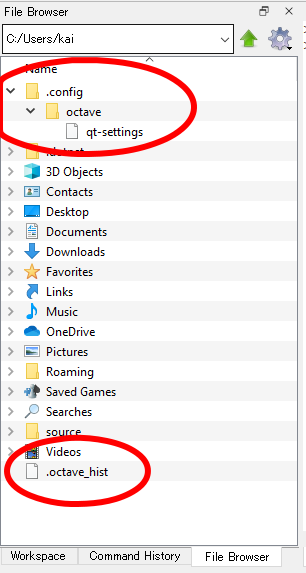
\includegraphics[width=\textwidth]{res/ms_windows/win_octave_settings.png}
\end{column}
\begin{column}{0.6\textwidth}
\begin{itemize}
\itemsep2em
\item
Setting files in User's home directory.

e.g. \texttt{C:\textbackslash Users\textbackslash kai}

\item
Delete them if GUI is not starting.

\item
Use/start Octave without GUI from other programs, see
\texttt{\small C:\textbackslash Octave\textbackslash
Octave-5.1.0.0\textbackslash
octave.vbs}
\end{itemize}
\end{column}
\end{columns}
\end{frame}

\end{document}
